\documentclass[letterpaper,twocolumn,openany,nodeprecatedcode]{dndbook}

% Use babel or polyglossia to automatically redefine macros for terms
% Armor Class, Level, etc...
% Default output is in English; captions are located in lib/dndstring-captions.sty.
% If no captions exist for a language, English will be used.
%1. To load a language with babel:
%	\usepackage[<lang>]{babel}
%2. To load a language with polyglossia:
%	\usepackage{polyglossia}
%	\setdefaultlanguage{<lang>}
\usepackage[italian]{babel}
%\usepackage[italian]{babel}
% For further options (multilanguage documents, hypenations, language environments...)
% please refer to babel/polyglossia's documentation.
\usepackage[utf8]{inputenc}
\usepackage[singlelinecheck=false]{caption}
\usepackage{lipsum}
\usepackage{listings}
\usepackage{shortvrb}
\usepackage{stfloats}
\usepackage{graphicx}% http://ctan.org/pkg/graphicx


\captionsetup[table]{labelformat=empty,font={sf,sc,bf,},skip=0pt}

\MakeShortVerb{|}

\lstset{%
  basicstyle=\ttfamily,
  language=[LaTeX]{TeX},
  breaklines=true,
}

\title{I corrieri della Grancontessa \\
\large OneShot di D\&D 5e per 4 o 6 giocatori di 4$^\circ$ livello}
\author{}
\date{2024/05/23}

\begin{document}

\frontmatter

\maketitle

\tableofcontents


\mainmatter%




%%%%%%%%%%%%%%% TEMPLATE %%%%%%%%%%%%%%%%%%%%%%%%

\chapter{Introduzione}

\section{Chi siamo}
\DndDropCapLine{C}{aro Dungeon Master}, siamo un gruppo di appassionati di D\&D che ha preparato questa avventura per te. Vorremmo condividere con te il nostro approccio al gioco di Dungeons \& Dragons per darti alcuni suggerimenti su come condurre al meglio questa avventura.

Quando creiamo i nostri personaggi, ci concentriamo sulla costruzione di personaggi complessi. Introduciamo difetti che possono aggiungere elementi divertenti al gioco, sviluppiamo background coerenti e integrati nell'ambientazione. Dedichiamo tempo a riflettere sui pensieri e le motivazioni dei personaggi, esplorando come reagirebbero a diverse situazioni. Ad esempio, durante la nostra ultima avventura, lo stregone Virgilio Monforte aveva problemi di memoria, mentre Clara Spina, la chierica, citava spesso proverbi senza senso. Prestiamo maggiore attenzione a questi aspetti rispetto alle regole specifiche di D\&D, che comunque consideriamo come punto di riferimento.

Quando un personaggio compie azioni che devono rimanere segrete dagli altri giocatori, utilizziamo Telegram per comunicare in modo riservato con il DM. Questa tecnica ha contribuito significativamente al divertimento di tutti in numerose occasioni. Nella OneShot descritta in questo testo, la comunicazione segreta con il DM è fondamentale per il successo dell'avventura.

Riteniamo che il DM debba avere una trama di base da seguire, ma sia importante saper improvvisare e adattarsi alle situazioni emergenti durante il gioco. Alla fine di questo testo, condivideremo un breve resoconto delle avventure vissute durante la nostra campagna.


\section{La oneshot}
Questa avventura è una OneShot del gioco di ruolo Dungeons \& Dragons\cite{dnd:giocatore}, progettata per un gruppo di 4-6 giocatori di 4$^\circ$ livello. L'ambientazione si colloca nel Medioevo Italiano, nei pressi del Castello di Canossa, i cui resti si trovano nel basso Appennino Reggiano, in Italia. Elementi magici, razze, classi e altri aspetti fantasy tipici di D\&D vengono integrati nell'ambientazione storica, ad eccezione delle seguenti razze non presenti: dragonidi, tiefling e mezz'orchi.

I personaggi giocanti (PG) sono creati dal Dungeon Master (DM). Nel paragrafo relativo al background dei PG (§\ref{PG}) sono fornite linee guida per la creazione dei personaggi. Alcuni di questi elementi sono considerati cruciali per mantenere coerenza con la trama. Inoltre, uno dei personaggi è un infiltrato nel gruppo con un'agenda segreta opposta a quella del resto del gruppo. Il DM dovrà gestire questa situazione e comunicare segretamente la missione al PG infiltrato.

La missione, inizialmente semplice e lineare, dovrebbe evolversi in un momento di conflitto interno al gruppo.

Le creature incontrate durante questa OneShot sono evidenziate in \textbf{grassetto} e fanno riferimento al Manuale dei Mostri di D\&D 5e\cite{dnd:mostri}.



\section{Contesto storico}

Matilde di Canossa\footnote{Questo paragrafo è stato dedotto e sintetizzato dalla voce enciclopedica di Wikipedia "Matilde di Canossa"} (Fig. \ref{fig:matilde})\cite{wiki:matilde}, o più correttamente Matilde di Toscana, nota anche con lo pseudonimo di \textit{Magna Comitissa} in italiano Gran Contessa, nacque nel 1046, terzogenita della potentissima famiglia feudale italiana dei Canossa considerata all'epoca la più potente famiglia d'Europa. Trascorse i primi anni della sua esistenza nell'agiatezza e serenità del castello di Canossa, teatro dei grandi banchetti e delle sontuose feste organizzate dal padre. Tuttavia a soli sei anni Matilde assistette a un evento che avrebbe cambiato radicalmente il corso della sua vita: il 6 maggio 1052 il padre Bonifacio fu ucciso a tradimento durante una battuta di caccia da uno dei suoi vassalli, che lo trapassò alla gola con una freccia avvelenata. L'agonia del duca durò alcune ore; nella tarda serata dello stesso giorno egli spirò.

\begin{figure}
\centering
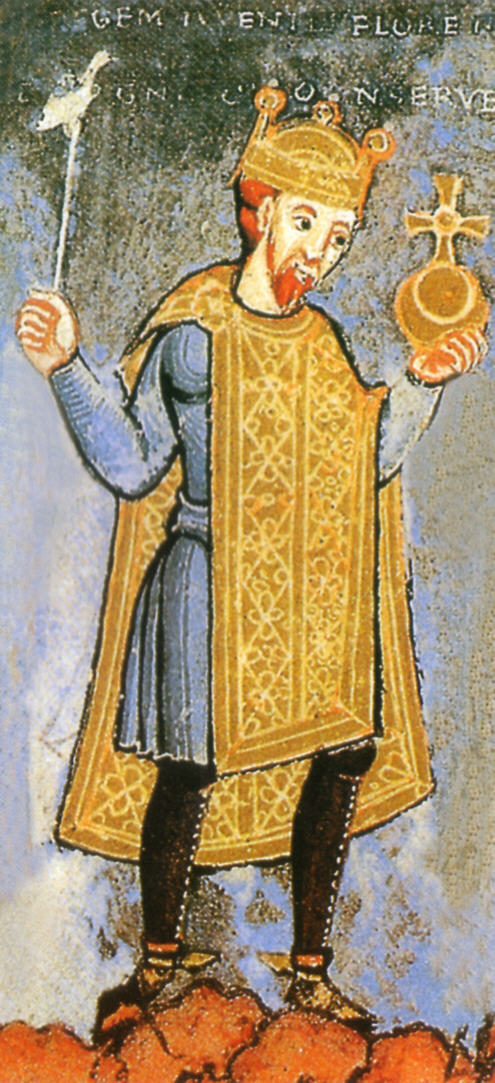
\includegraphics[width=9cm]{./img/enrico3.png}
\caption{Riproduzione di Enrico III. Immagine di Pubblico Dominio da Wikimedia Commons.}
\label{enrico3}
\end{figure}


Beatrice, la madre di Matilde, rimasta vedova con 3 figli piccoli in difficoltà nel reggere il ruolo del marito Bonifacio, capo di una casata così potente, cercò la protezione dell'imperatore Enrico III (Fig. \ref{enrico3}) il quale garantì questo privilegio per Matilde e i suoi fratelli.

Purtroppo i fratelli di Matilde perirono per un maleficio: avvelenamento.

La madre di Matilde era imparentata con il papa Leone IX che garantiva anch'egli una protezione alla casata dei Canossa. Gli equilibri fra potere temporale e potere spirituale permisero alla giovane Matilde e alla sua casata di trascorrere alcuni anni in relativa serenità.

Alla morte del papa Leone IX cambiarono gli equilibri e l'imperatore Enrico III prese in ostaggio Matilde e sua madre e le portò in Germania; ma dopo un anno anche Enrico III morì e così Matilde ritornò in Italia. La madre Beatrice cercò una nuova protezione risposandosi con Goffredo il Barbuto.

Goffredo il Barbuto, sposando Beatrice, era diventato signore della Tuscia. Una clausola del contratto di matrimonio stabilì che il figlio di Goffredo, detto Goffredo il Gobbo (Fig. \ref{fig:goffredo}), avrebbe sposato la figlia di Beatrice, Matilde, per consolidare il suo potere e quello dei Canossa.

Matilde e Goffredo il Gobbo si unirono in matrimonio nella Lorena Francese. Il marito era un giovane onesto e coraggioso, ma afflitto da alcuni difetti fisici (tra gli altri gozzo e gobba), comunque Matilde, conscia dei doveri nobiliari per i quali era stata educata e con la persuasione della madre, seppur riluttante restò in Francia coabitando con il marito e ne rimase incinta.

All'inizio del 1071 Matilde partorì una bambina che chiamò Beatrice, per poter rinnovare il nome della madre. Il parto però non fu facile e dopo pochi giorni la piccola Beatrice morì. La mamma di Matilde eresse il monastero di Frassinoro, nell'Appennino Modenese, per <<la grazia dell'anima della defunta Beatrice mia nipote>>.

Nei mesi successivi Matilde rischiò la vita, non solo per i postumi del parto difficile, ma anche per l'ira del casato di Lorena che accusò la Gran Contessa di portare il malocchio. Nel gennaio del 1072 Matilde fuggi dalla Lorena Francese per tornare nel Castello di Canossa con la madre.

Il 26 dicembre del 1073 i PG sono stati incaricati da Tobaldo Malatesta\footnote{Questo NPC non è realmente esistito}, fedele servitore di Matilde, di condurre un carro di provviste (salumi, formaggi, grano e vino) da Parma al Castello di Canossa entro il 28 dicembre. Inoltre è stata consegnata al paladino del gruppo  una pergamena, una cosiddetta \textit{rotula}, che dovrà consegnare personalmente a Matilde, proteggendo la segretezza della missiva a costo della vita. La rotula di pergamena è avvolta in una pezzo di pelle e sigillata con il simbolo di cera lacca della casata dei Canossa. 

\begin{figure}
\centering
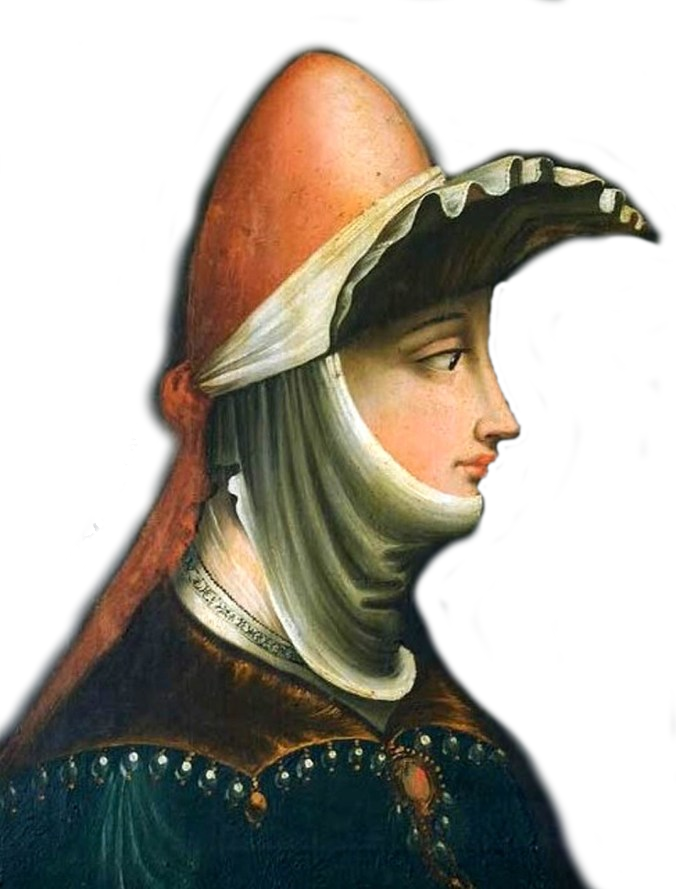
\includegraphics[width=7.5cm]{img/matilde.png}
    \caption{\textsf{Parmigianino, Ritratto di Matilde di Canossa, XVI secolo, Museo Diocesano, Mantova}}
    \label{fig:matilde}
\end{figure}

\begin{DndSidebar}{Quando fornire queste informazioni?}Il contesto storico descritto in questo paragrafo può essere presentato ai giocatori dal Dungeon Master nel momento ritenuto più opportuno. Durante la nostra partita a questa avventura, il DM ha utilizzato un avventore della locanda per trasmettere queste informazioni ai PG.
\end{DndSidebar}

\subsection{Eventi successivi}
A parte la missione dei PG e il personaggio di Tobaldo Malatesta, gli eventi storici menzionati sono realmente accaduti. Di seguito viene descritto ciò che accadde a Matilde dopo il suo ritorno al Castello di Canossa. Questi avvenimenti non fanno parte dell'avventura stessa, ma possono essere utili per il DM che desidera preparare questa OneShot, al fine di comprendere meglio il concetto alla base della storia.

Tra il 1073 e il 1074, il marito di Matilde, Goffredo il Gobbo, scese in Italia per riconquistarla offrendole terre e armate, ma la Grancontessa rispose con fermezza e determinazione. Il suo atteggiamento contribuì a creare il mito di una donna priva di debolezze.

Nel 1076, Goffredo il Gobbo cadde vittima di un'imboscata nelle sue terre vicino ad Anversa. Durante la notte, mentre si recava al gabinetto, un sicario in agguato gli conficcò una spada tra le natiche, lasciando l'arma conficcata nella ferita. Inizialmente sembrava che potesse sopravvivere, ma una settimana dopo, il 27 febbraio 1076, morì, lasciando Matilde vedova. Molti commentatori dell'epoca la accusarono di essere stata personalmente coinvolta nel crimine; tuttavia, il colpevole più probabile fu indicato come il conte fiammingo Roberto I delle Fiandre. In ogni caso, Matilde non offrì alcun sostegno finanziario alla Chiesa per l'anima del marito ucciso, né fece celebrare una messa o dedicò un convento in suo onore, come era consuetudine tra i nobili.

\begin{figure}
\centering
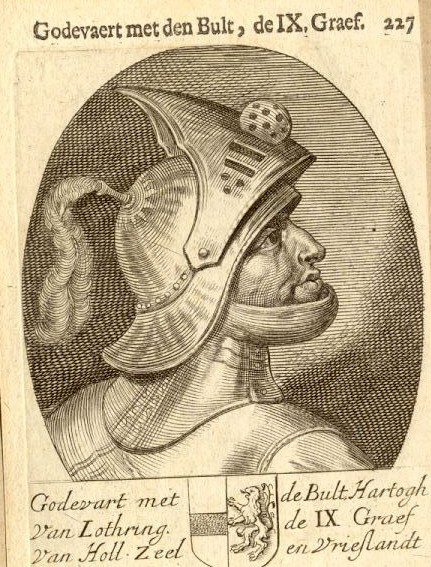
\includegraphics[width=7.5cm]{img/goffredo-il-gobbo.png}
    \caption{\textsf{Goffredo IV di Lorena detto ''il Gobbo''}}
    \label{fig:goffredo}
\end{figure}

\section{La missione}
È il 26 dicembre del 1073, i PG si trovano nella città di Parma dove sono stati incaricati da Tobaldo Malatesta, servitore di alto rango della casata dei Canossa, di scortare un carro di provviste destinate al Castello di Canossa. Il carro contiene prosciutti, salami, culatelli e forme di formaggio stagionato, che gli abati Benedettini di Parma hanno iniziato a produrre da alcuni mesi\footnote{L'origine del Parmigiano reggiano, secondo la voce enciclopedica di Wikipedia, avrebbe origine nel XII secolo nelle abbazie benedettine e cistercensi situate fra Reggio Emilia e Parma. Ci sembrava carino aggiungere a questa storia le origini del formaggio più famoso del mondo anche se in realtà nacque un po' dopo.}, destinati alla festa di fine anno che si svolgerà al castello. Oltre ai viveri Tobaldo consegna una pergamena sigillata al paladino del gruppo, Dante Passafiume, che dovrà portare personalmente a Matilde e dovrà proteggerne la segretezza anche a costo della propria vita.

Herbert Mann, il cui vero nome è Olin, avrà una missione segreta diversa. Questo PG è un sicario incaricato da Roberto I delle Fiandre il quale lo ha pagato in anticipo 200 monete d'oro per uccidere Goffredo il Gobbo, \textbf{nobile} con 32 PF (Manuale dei Mostri p.349 \cite{dnd:mostri}) che alloggia al Castello di Canossa. Il sicario è riuscito ad infiltrarsi nel gruppo di corrieri per il trasporto di viveri al Castello, tuttavia la sua missione è una missione omicida.


\section{PG in breve}\label{PG}

\paragraph{Isabella Grattaciotoli} Ha 28 anni, è una \textit{halfling ladra}. Non particolarmente forte ma molto abile a nascondersi e particolarmente agile. Orfana di entrambi i genitori ha accettato di partecipare a questa missione perché la ricompensa le parmetterà di provvedere al sostegno dei suoi fratelli per tutto l'inverno. Difetti: quando vede dei dolci perde letteralmente la testa.

\paragraph{Dante Passafiume} (PG indispensabile) È un \textit{paladino umano} di 50 anni, un veterano che fa parte della rete di messaggeri. Una persona coraggiosa e dall'alta integrità morale. Dante, se prende un impegno, lo porta a termine. Difetti: si irrita quando viene contraddetto.

\paragraph{Caterina Portinari} Caterina ha 25 anni ed è la più giovane del gruppo. Viene da una famiglia benestante. I genitori avrebbero voluto educarla per diventare una signora, una damigella, ma lei è una donna di azione. Fuggita dalla famiglia, ha studiato per un paio d'anni armi e tattiche di cobattimento e ora è un'abile \textit{guerriera umana}. Difetti: quando si tratta di finire un nemico esita.

\paragraph{Virgilio Monforte} È uno \textit{stregone mezz'elfo} anziano di 132 anni. Ha sempre messo i suoi innati poteri al servizio dei nobili del territorio. Difetti: a volte perde la testa e usa incantesimi totalmente inutili.

\paragraph{Clara Spina} Clara ha 35 anni, è una umana chierica, appartiene al dominio della vita, la sua missione è aiutare gli altri. Difetti: è una irrefrenabile pettegola.

\paragraph{Olin (nome di copertura Herbert Mann)} (PG indispensabile) È un \textit{umano ladro} di 43 anni ma ufficialmente bardo con uno strumento rotto. È un sicario infiltrato nel gruppo per uccidere Goffredo il Gobbo. Difetti: è irritato dai nobili altezzosi, anche se riesce a trattenersi, a volte la sua irritazione traspare.




\subsection{NPC in breve}

\paragraph{Tobaldo Malatesta} Servitore di alto rango di Matilde. Gentile, una persona abituata a comandare, conosce Dante Passafiume.

\paragraph{Filippo Pocaterra} Oste della Locanda del cane zoppo di San Polo. Gentile ma non è la persona più pulita del regno. L'igiene non è la sua specialità.

\paragraph{Desiderio Forgiaferro} Mago anziano estremamente gentile e servizievole, brama di tradire Matilde e vorrebbe ingraziarsi i suoi nemici sperando di ricevere maggiore fortuna economica.

\paragraph{Matilde di Canossa} La Grancontessa ha 25 anni, ha la fama di essere una donna dura tutta di un pezzo, ma probabilmente è più debole di quello che sembra.

\paragraph{Goffredo il Gobbo} Ha una vistosa gobba ma di fatto è una persona massiccia che sa difendersi. Non è la persona più simpatica del mondo. È venuto in Italia per riconquistare Matilde promettendole terre. Quest'ultima lo ha rifiutato. Considera Matilde una lurida sgualdrina.


\chapter{L'arrivo al villaggio}
\DndDropCapLine{I}{ PG stanno trasportando} un carico di viveri e una pergamena con un messaggio segreto da consegnare di persona a Matilde. La missiva è in custodia al paladino che deve difenderla a costo della vita. Il DM potrebbe decidere di non rivelare subito la missione e leggere il testo seguente.

\begin{DndReadAloud}
Siamo nell'anno del Signore 1073. Oggi è il 26 dicembre. L'inverno è iniziato da poco ma sta già colpendo duramente. La neve cade spinta dal vento in tutte le direzioni come in una vera bufera. Sono le 5 del pomeriggio il sole che non si è visto per tutto il giorno è da poco sceso all'orizzonte e il grigio del cielo si sta trasformando rapidamente in nero. Una giornata ideale per mettersi seduti con i piedi al calduccio davanti al camino e mangiarsi una ciotola di stufato di maiale sotto una calda coperta. Purtroppo la sorte aveva altri piani per voi. Vi trovate nella tormenta a scortare un carro nella nebbia, nel turbinare della neve e con il buio che avanza con rapidità.

Clara Spina, la vostra chierica, conduce il carretto trainato da un mulo stanco che arranca nella neve alta una ventina di centimetri. Al fianco di Clara è seduto Virgilio Monforte, uno stregone. Virgilio ha lo sguardo perso e la sua mente sta viaggiando lontano. Forse in un luogo caldo? O magari nel luogo dove ha acquisito i suoi innati poteri. Davanti al carro Dante Passafiume, il vostro paladino conduce il gruppo ed è scortato, da Herbert Mann, un giovane bardo, che lo segue a pochi metri di distanza. 
\end{DndReadAloud}

Il gruppo arriva al fiume e scorgono il primo villaggio.

\begin{DndReadAloud}
Il carro procede a rilento, le ruote faticano ad affondare nella neve. Davanti a voi scorgete un ponte in legno dall'aspetto robusto, oltre il ponte fanno capolino le luci di un piccolo villaggio: \textit{Plebs de Caviliano}. La vostra comitiva avanza. Dante testa la robustezza del ponte, ma non ha motivo di dubitare: da queste parti, quando costruiscono qualcosa, lo fanno a regola d'arte. Percepite di essere sul ponte poiché il rumore sordo delle ruote del carro e del vostro mulo rimbomba leggermente sulle robuste assi di legno. Alcuni di voi hanno già attraversato questo fiume e lo conoscono molto bene. Clara in estate vi faceva il bagno con la sorella, Dante lo ha attraversato per lavoro decine di volte e Virgilio... bhe purtroppo Virgilio ha un brutto ricordo ricordo legato a questo fiume e non ne ha mai parlato con nessuno. Herbert, lo straniero del gruppo, è la prima volta che lo attraversa. Un fiume che oggi sembra scomparso perché scorre sotto una coltre di ghiaccio ricoperto da uno strato di neve. Si tratta del Fiume Enza e, come vi dicevo, il villaggio di fronte a voi è  \textit{Plebs de Caviliano} che ai giorni nostri è noto come San Polo.
\end{DndReadAloud}

A questo punto probabilmente i PG si staranno chiedendo cosa trasportano.

\begin{DndReadAloud}
Vi starete chiedendo cosa trasporta il vostro carro. Si tratta di un carro abbastanza grande coperto da un pesante tendone per proteggere la merce trasportata. Per capire cosa trasporta il carro dobbiamo tornare indietro di qualche ora, nella città di Parma, dove avete incontrato Tobaldo Malatesta, servitore di alto rango della casata dei Canossa. Tobaldo è una persona gentile ed evidentemente abituata al comando, vi ha incaricato di trasportare un carico di viveri al castello di Canossa al quale dovete arrivare entro il 29 di dicembre. Il carro contiene cosce di maiale stagionate, salami di maiale e culatelli prodotti dai lardaroli di Parma; svariate caciotte e una grossa forma di formaggio stagionato che il monastero benedettino di San Giovanni Evangelista ha provato a produrre lo scorso anno e sembra essere molto buono. Questo goloso carico servirà per la festa di fine anno che si volgerà al castello.

Tobaldo ha poi preso in disparte il vostro paladino per consegnargli una pergamena che Dante Passafiume dovrà consegnare personalmente a Matilde. Tobaldo, posando una mano sulla spalla di Dante ha pronunciato alcune parole che tutto il vostro gruppo ha potuto sentire <<Mio caro Dante, appartieni da alcuni anni alla rete dei messaggeri e la tua fama in ti precede ovunque tu vada. Custodisci la segretezza di questa missiva destinata alla Grancontessa a costo della tua stessa vita e comanda il tuo gruppo per raggiungere il tuo obiettivo>>
\end{DndReadAloud}

Nel pomeriggio, dopo aver ricevuto l'incarico da Tobaldo, il gruppo è partito nella tormenta per raggiungere l'abitato di San Polo dove fare tappa.


\DndFeatHeader{Il carro al sicuro}
All'arrivo al villaggio di San Polo i PG saranno costretti ad alloggiare alla locanda per trascorrere la notte ed eventualmente attendere il passaggio della tormenta. Nella locanda troveranno alcuni NPC che racconteranno quanto il DM vorrà della storia riportata all'inizio del presente testo.

\begin{DndReadAloud}
Quando entrate nella locanda affollata, il brusio di abbassa istantaneamente e alcuni ospiti si girano per osservarvi incuriositi. La maggior parte di loro sono contadini. All'ingresso un misto di odore stufato, legna bruciata, letame e sudore arriva alle vostre narici. L'oste vi fa un caloroso sorriso dietro ai suoi baffoni.
\end{DndReadAloud}

L'oste, Filippo Pocaterra (\textbf{popolano}), darà il massimo delle rassicurazioni ai PG garantendo che nessuno potrà toccare i viveri presenti sul carro in quanto saranno posizionati in una stalla che verrà chiusa con un pesante lucchetto.




\DndFeatHeader{NPC della locanda}
Alla locanda sono presenti alcuni abitanti della zona, per lo più contadini. Il DM potrebbe aggiungere eventuali PG che non partecipano alla OneShot tenendo conto del loro background. Ad esempio la cameriera potrebbe essere Isabella Grattaciotoli.

Alla locanda potranno parlare con persone della zona che li informeranno sul fatto che circola voce che Goffredo il Gobbo sia giunto dalla Francia per andare al Castello di Canossa per riconquistare Matilde. Se i PG non sono ancora stati informati sui fatti storici passati e che significato abbia la visita di Goffredo il Gobbo, il DM dovrebbe interpretare gli NPC per fornire ai giocatori le informazioni descritte nell'inquadramento storico.

\DndFeatHeader{Il pasto}
L'oste offrirà loro una camera agiata è una sostanziosa cena al costo di 8 ma. Per la cena potranno scegliere fra stufato di maiale o pollo alla cacciatore e una caraffa di vino rosso.

I PG che mangeranno lo stufato di maiale, prima di coricarsi, dovranno fare un TS su costituzione con CD 11, se non lo superano, si ammalano di \textit{Epidemia fognaria} (Manuale del DM, p.257 \cite{dnd:dm})). I PG ammalati passeranno la notte vomitando e, il giorno dopo saranno Indeboliti al livello 1 (Manuale del Giocatore p.291 \cite{dnd:giocatore}). Alla mattina potranno rifare un TS su costituzione per vedere se l'indebolimento peggiora o migliora. Al termine di ogni riposo lungo successivo, potranno rifare il TS per vedere se la malattia si aggrava o no, non potranno recuperare PF ma potranno tirare un dado vita ogni riposo breve di almeno 1 ora aggiungendo metà del punteggio ottenuto.

\begin{DndTable}[color=PhbLightCyan,header=Indebolimento]{cX}
  \textbf{Liv.} & \textbf{Effetto} \\
  1 & Svantaggio alle prove di caratteristica \\
  2 & Velocità dimezzata \\
  3 & Svantaggio ai tiri per colpire e ai TS \\
  4 & Massimo dei punti ferita dimezzato \\
  6 & Velocità ridotta a 0 \\
  7 & Morte \\
\end{DndTable}






\chapter{Verso Canossa}
\DndDropCapLine{L}{a tormenta è passata.} I PG si risvegliano in una limpida giornata ivernale. L'aria è gelida e luminosa e il paesaggio è completamente ammantato di bianco. Guardando a Nord sono in grado di vedere la foresta che si estende nella pianura e in fondo sono debolmente visibili le Alpi anche loro ammantate di neve.

Quando i PG partiranno alla volta del Castello di Canossa, potranno scegliere due strade: portarsi verso Quattrocastella e salire a Canossa oppure proseguire lungo la valle dell'Enza e poi salira a Est verso Canossa.

\section{Banditi}
I PG troveranno sul terreno un finto cadavere. Quando scenderanno dal carro saranno circondati da 2 \textbf{banditi} più il \textbf{capo dei banditi}.

\section{Il mago traditore}
Mentre i PG viaggiano verso il castello di Canossa, scorgono davanti a loro delle impronte nella neve sono impronte di umano. Se indagano possono scoprire che l'umano ha un bastone e trascina un piede.

L'umano è uno dei consiglieri di Matilde diretto a Canossa. Si tratta di un \textbf{mago} (Manuale dei Mostri p.348 \cite{dnd:mostri}) che ha tutta l'intenzione di tradire Matilde. 

\begin{DndSidebar}{Interpretare il mago}
Il mago è vecchio e affaticato. Deve far credere ai PG che se prosegue nella neve rischia di morire. Racconterà che è stato rapinato dai banditi che gli hanno rubato il mulo e tutti i suoi averi. È diretto al castello perché è stato invitato da Matilde come consigliere per la festa di fine anno.
\end{DndSidebar}

Il mago è stato informato che un certo numero di avventurieri è stato incaricato di portare un carico di viveri a Canossa. Uno di questi avventurieri ha un messaggio segreto, non sa chi sia il messaggero.

Per prima cosa proverà a capire se sono il gruppo di avventurieri che trasporta il cibo a Canossa.

Se capirà che sono loro proverà a lanciare l'incantesimo \textit{suggestione} all'halfling del gruppo parlandole in halfling.


\begin{DndReadAloud}
Mia cara, era da molto che non vedevo un halfling da queste parti. Da dove provieni?
Saresti così gentile da fare una cosa per me? Mia cara, mi risulta che state trasportando un messaggio per Matilde. Quando ritieni più opportuno dovresti leggere il messaggio e riferirmi il contenuto. TS 14
\end{DndReadAloud}


\section{Udienza con Matilde}
Quando i PG stanno per arrivare al Castello di Canossa, descrivi quanto segue.

\begin{figure}
\centering
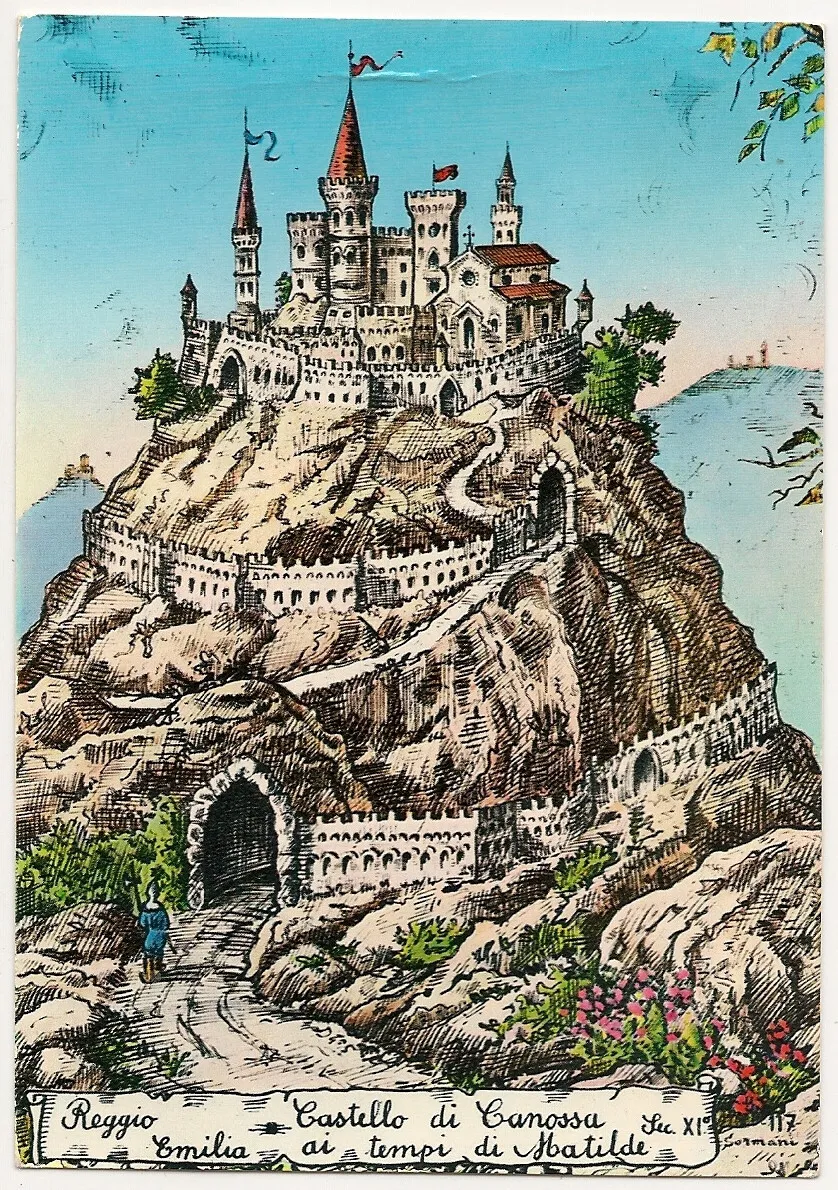
\includegraphics[width=7.5cm]{img/castello.png}
\caption{Il Castello di Canossa riprodotto in una cartolina pubblicata e in vendita su eBay}
\label{castello}
\end{figure}


\begin{DndReadAloud}
Mentre il carro tirato dal povero animale da soma procede lungo la mulattiera ogni tanto scorgente su promontorio di arenaria sul quale sorge il maestoso Castello di Canossa. Mano a mano che procedete uscite dal bosco e potete scorgere l'intero paesaggio della zona. Nelle colline vicine a Canossa, in questa bella giornata di inverno, scorgete su una collina vicina la fortezza difensiva di Canossa: Rossena con la sua torre di guardia che molti chiamano Rossenella.

Quanto arrivate alla residenza di Matilde, alle porte delle mura che conducono al promontorio due guardie vi intimano di fermarvi. <<Alt! Chi siete? Cosa volete? Cosa portate?>>
\end{DndReadAloud}

\bibliography{bibliografia}{}
\bibliographystyle{plain}

\end{document}

